% --------------------------------------------------------------
% This is all preamble stuff that you don't have to worry about.
% Head down to where it says "Start here"
% --------------------------------------------------------------
 
\documentclass[12pt]{article}
 
\usepackage[margin=1in]{geometry} 
\usepackage{amsmath,amsthm,amssymb,mathtools}
\usepackage{dsfont} % for indicator function \mathds 1
\usepackage{tikz,pgf,pgfplots}
\usepackage{enumerate} 
\usepackage{graphicx,float} % figures
\usepackage{csvsimple,longtable,booktabs} % load csv as a table
\usepackage{listings,color} % for code snippets

\newenvironment{theorem}[2][Theorem:]{\begin{trivlist} %% Theorem Environment
\item[\hskip \labelsep {\bfseries #1}\hskip \labelsep {\bfseries #2.}]}{\end{trivlist}}

\newtheorem{definition}{Definition}
\let\olddefinition\definition
\renewcommand{\definition}{\olddefinition\normalfont}
\newtheorem{lemma}{Lemma}
\let\oldlemma\lemma
\renewcommand{\lemma}{\oldlemma\normalfont}
\newtheorem{proposition}{Proposition}
\let\oldproposition\proposition
\renewcommand{\proposition}{\oldproposition\normalfont}
\newtheorem{corollary}{Corollary}
\let\oldcorollary\corollary
\renewcommand{\corollary}{\oldcorollary\normalfont}

\newcommand\norm[1]{\left\lVert#1\right\rVert} % \norm command 

\pgfmathsetseed{26}
\newcommand{\Emmett}[5]{% points, advance, rand factor, options, end label
\draw[#4] (0,0)
\foreach \x in {1,...,#1}
{   -- ++(#2,rand*#3+0.001)
}
node[right] {#5};
}

\begin{document}
 
% --------------------------------------------------------------
%                         Start here
% --------------------------------------------------------------
 
\title{Mathematical \& Computational Finance II\\Lecture Notes}
\author{Welcome to Measure Theory}
\date{September 22 2015 \\ Last update: \today{}}
\maketitle

\begin{section}{Continue the Crash Course on Probability Measures}

\begin{definition} \label{def:norm} For $X \in L^p(\Omega \mathcal F, \mathbb P)$, for $1 \leq p < \infty$, define a \underline{norm} (generalized Euclidean norm on $\mathbb R^n$) as
\begin{equation*}
	\norm{X}_p = (\mathbb E|X|^p])^{^1/_p}
\end{equation*}
\end{definition}

\noindent Let $1 \leq p < \infty$, define $q = \frac{p}{1-p}$~\footnote{That is, $q$ is the conjugate to $p$.}. Then $q \in (1, \infty)$ and $\frac{1}{p} + \frac{1}{q} = 1$. If $p$ and $q$ are conjugates then, for $a, b > 0$,
\begin{equation*}
	a^{^1/_p} + b^{^1/_q} \leq \frac{1}{p}a + \frac{1}{q}b
\end{equation*}

\begin{proposition} If $p$ and $q$ are conjugates and $X \in L^p, Y \in L^q$ then,
\begin{align*}
	XY &\in L^1 \quad \text{and} \\
	\mathbb E[|XY|] &\leq \norm{X}_p + \norm{Y}_p
\end{align*}
\end{proposition}

\begin{proposition} (Minkowski's Inequality)\footnote{This is a generalization to the Triangle Inequality.} For $1 \leq p < \infty$, if $X, Y \in L^p$ then
\begin{align*}
	X + Y& \in L^p \quad \text{and} \\
	\norm{X + Y}_p &\leq \norm{X}_p + \norm{Y}_p
\end{align*}
\end{proposition}

\noindent \underline{Remarks}:
\begin{enumerate}
	\item $\norm{\lambda X}_p = \lambda\norm{X}_p$, for $\lambda \in \mathbb R$
	\item $\norm{X + Y}_p \leq \norm{X}_p + \norm{Y}_p$
	\item If $\norm{X}_p = 0$ then $|X|_p = 0$ a.s. $\implies X = 0$ a.s.\footnote{i.e. $X = 0$ up to an equivalence class a.s.}
\end{enumerate}
These remarks give us that $\norm{\cdot}_p$ is a \underline{norm} on $L^p$. So, we say that $L^p$ is a \underline{normed linear space}.

\subsection{$L^2$ and Conditional Expectation}

A linear functional on $L^2$ is a map $\phi : L^2(\Omega, \mathcal F, \mathbb P) \rightarrow \mathbb R$, or equivalently $\phi : X \rightarrow \mathbb R$, such $\phi$ is linear:
\begin{equation*}
	\phi(\alpha X + \beta Y) = \alpha\phi(X) + \beta\phi(Y) \quad \forall\,X,Y \in L^2,\forall\,\alpha,\beta\in\mathbb R
\end{equation*}
A map $\phi: L^2 \rightarrow \mathbb R$ is \underline{bounded} if $\exists\,k>0$ such that
\begin{equation*}
	|\phi(X)| \leq k\norm{X}_2 \quad \forall\,X\in L^2
\end{equation*}

\noindent A sequence of random variables $\{X_n\} \in L^p$ converges to $X \in L^p$ if
\begin{align*}
	&X \in L^p \quad \text{and} \\
	\norm{X_n - X}_p &\longrightarrow 0 \quad \text{as $n \longrightarrow \infty$}
\end{align*}

\noindent Suppose $\{X_n\} \in L^2$ converges to $X \in L^2$ and $\phi$ is a bounded linear functional on $L^2$ then,
\begin{align*}
	|\phi(X_n) - \phi(X)| &= |\phi(X - X_n)| \quad \text{(by linearity)} \\
	|\phi(X_n - X)| &\leq k\norm{X_n - X}_2 \longrightarrow 0 \quad \text{(as $n \longrightarrow \infty$)}
\end{align*}

\noindent Now we may define
\begin{definition} Suppose $\phi$ is a bounded linear functional on $L^2$, define
\begin{equation*}
	\norm{\phi} = \inf_{\{X \in L^2\,:\,\norm{X}_2 \neq 0\}} \frac{|\phi|}{\norm{X}_2}
\end{equation*}
\end{definition}

\noindent \underline{Aside}: $L^2(\Omega,\mathcal F,\mathbb P)$ is what we call a {\em Hilbert Space}\footnote{A Hilbert Space is a {\em complete} inner product space (Banach Space)\footnotemark.}\footnotetext{Left undefined for this course.} with inner product
\begin{equation*}
	\langle X,Y \rangle = \int XY\, d\mathbb P = \mathbb E[XY]
\end{equation*}

\begin{definition} A sequence $\{Y_n\}$ in a normed vector space is a \underline{Cauchy sequence} if 
\begin{equation*}
	\sup_{m \in N} \norm{y_{n+m} - y_n} \longrightarrow 0 \quad \text{as $n \longrightarrow \infty$}
\end{equation*}
That is, we take elements of the sequence arbitrarily far apart and see their norm $\longrightarrow 0$ as $n \longrightarrow 0$.
\end{definition}

\noindent We say a space is \underline{complete} if every Cauchy sequence is a convergent sequence.

\begin{theorem}{$L^p(\Omega, \mathcal F, \mathbb P)$ is a complete normed vector space}
\end{theorem}

\noindent Why is this important? Whenever you have a Hilbert space this gives you the following theorem...

\begin{theorem}{Riesz Representation Theorem} Let $\mathcal H$ be a Hilbert space and $L$ be a linear continuous functional on $\mathcal H$. Then there exists a unique $y \in \mathcal H$ such that
\begin{equation*}
	L(x) = \langle x,y\rangle \quad \forall x,y\in\mathcal H \quad \text{with } \norm{L} = \norm{y}
\end{equation*}
\end{theorem}

\begin{definition} \label{def:condexpect} Let $X \in L^2(\Omega, \mathcal F, \mathbb P)$ and $\mathcal G \subseteq \mathcal F$ (i.e. $\mathcal G$ is a sub-$\sigma$-algebra of $\mathcal F$). Then the \underline{conditional expectation} of $X$ with respect to $\mathcal G$ denoted $\mathbb E[X|\mathcal G]$ is a random variable $Z \in L^2$ satisfying
\begin{enumerate}
	\item $Z$ is $\mathcal G$-measurable. \label{gmeasurable}
	\item $\mathbb E[ZY] = \mathbb E[XY] \quad \forall$ bounded $\mathcal G$-measurable random variables $Y$. \label{ezy=exy}
\end{enumerate}
Note that $Z$ is a random variable depending on $\omega \in \Omega$ meaning $Z = Z(\omega) = \mathbb E[X|\mathcal G](\omega)$.
\end{definition}

\subsubsection{Existence} For fixed $X\in L^2(\Omega,\mathcal F,\mathbb P)$ the map 
\begin{align*}
&\phi_X : L^2(\Omega, \mathcal F, \mathbb P) \rightarrow \mathbb R \quad \text{or equivalently} \\
&\phi_X : Y \rightarrow \mathbb E[XY]
\end{align*}
is a bounded continuous linear functional on $L^2(\Omega, \mathcal G, \mathbb P)$. So,
\begin{equation*}
	\exists\,Z \in L^2(\Omega, \mathcal G, \mathbb P) \quad \text{(by the Riesz Representation Theorem)}
\end{equation*}
Such that
\begin{equation*}
	\phi_X(Y) = \int XY\,d\mathbb P = \langle Z, Y\rangle = \int ZY\,d\mathbb P
\end{equation*}
For all $Y \in L^2(\Omega, \mathcal G, \mathbb P)$. \\
$\therefore Z$ satisfies Definition \ref{def:condexpect} Conditions \ref{gmeasurable} and \ref{ezy=exy}. 

\subsubsection{Uniqueness} This is trickier to do and is omitted in this course.

\subsubsection{Interpretation} $\mathbb E[X_2|X_1]$ {\em really} means $\mathbb E[X_2 | \sigma (X_1)]$ where the conditional $\sigma(X_1)$ means the information generated by the smallest $\sigma$-algebra generated by $X_1$.

\subsubsection{Properties} 
\begin{enumerate}
	\item Linear: $\mathbb E[\alpha X_1 + \beta X_2 | \mathcal G] = \alpha \mathbb E[X_1|\mathcal G] + \beta\mathbb E[X_2|\mathcal G]$
	\item Integrable: $\mathbb E[|\mathbb E[X|\mathcal G]|] < \infty$
	\item If $X \geq 0$ then $\mathbb E[X|\mathcal G] \geq 0$ (in probability a.s.)
	\item $\mathbb E[a|\mathcal G] = a, \quad \forall\,a\in\mathbb R$
	\item ``Taking out what is known'': If $W$ is $\mathcal G$-measurable (i.e. $W \in \mathcal G$) and $\mathbb E[|XW|] < \infty$ (i.e. XW is integrable) $\implies \mathbb E[XW|\mathcal G] = W\mathbb E[X|\mathcal G]$
\begin{corollary} If $X$ is $\mathcal G$-measurable then $\mathbb E[X|\mathcal G] = X$
\end{corollary}
\begin{corollary} If $X$ is independent\footnote{$X$ is independent of $\mathcal G$ if $\forall\,A\in\sigma(X)$ and $\forall\,B\in\mathcal G \implies \mathbb P(A\cap B) = \mathbb P(A)\mathbb P(B)$. This is something to absorb \& dwell on for a moment... but the basic intuition is the same.}~of $\mathcal G$ then $\mathbb E[X|\mathcal G] = \mathbb E[X]$ (i.e. $\mathcal G$ gives us no information about $X$).
\end{corollary}
Remember: If $\mathcal C$ generates $\mathcal F$ then $\{X^-1(c):c\in\mathcal C\}$ generates $\sigma(X)$.
	\item The ``Tower' Property'': If $\mathcal H \subseteq \mathcal G$ are sub-$\sigma$-algebras of $\mathcal F$ then
		\begin{align*}
			\mathbb E[\mathbb E[X|\mathcal G]|\mathcal H] &= \mathbb E[X|\mathcal H] \\
			&= \mathbb E[\mathbb E[X|\mathcal H]|\mathcal G]
		\end{align*}
	\item ``Jensen's Inequality'': If $X \in L^2$ we can show
		\begin{equation*}
			(\mathbb E[X|\mathcal G])^2 \leq \mathbb E[X^2|\mathcal G]
		\end{equation*}
\end{enumerate}

\noindent Here's a nice result as to why conditional expectation is useful
\begin{proposition} Let $X \in L^2, g(Y) \in L^2$ (i.e. $g$ is a square integrable function) then
	\begin{align*}
		\mathbb E[(X - g(Y))^2] &= \int (X - g(Y))^2\,d\mathbb P \\
		&= \int (X - \mathbb E[X|\sigma(Y)] + \mathbb E[X|\sigma(Y)] - g(Y))^2\,d\mathbb P \quad \text{(add \& subtract the same value)} \\
		&= \int (X - \mathbb E[X|\sigma(Y)])^2\,d\mathbb P + 2\int (X - \mathbb E[X|\sigma(Y)])(\mathbb E[X|\sigma(Y)] - g(Y))\,d\mathbb P \\
		&\hphantom{{} = \int (X - \mathbb E[X|\sigma(Y)])^2\,d\mathbb P + 2\int (X - } + \int (\mathbb E[X|\sigma(Y)] - g(Y))^2\,d\mathbb P  \\
		&= \mathbb E[(X - \mathbb E[X|\sigma(Y)])^2]+ 2\mathbb E[(X - \mathbb E[X|\sigma(Y)])(\mathbb E[X|\sigma(Y)] - g(Y))] \\
		&\hphantom{{} = \mathbb E[(X - \mathbb E[X|\sigma(Y)])^2]+ 2\mathbb E[(X - } + \mathbb E[(\mathbb E[X|\sigma(Y)] - g(Y))^2] \\
	\end{align*}
Note that in the middle term $\mathbb E[(X - \mathbb E[X|\sigma(Y)])(\mathbb E[X|\sigma(Y)] - g(Y))]$ we have $(\mathbb E[X|\sigma(Y)] - g(Y)) \in \sigma(Y)$, so
	\begin{align*}
		\mathbb E[(X - \mathbb E[X|\sigma(Y)])(\mathbb E[X|\sigma(Y)] - g(Y))]  &= \mathbb E[\{(X - \mathbb E[X|\sigma(Y)])(\mathbb E[X|\sigma(Y)] - g(Y))\}|\sigma(Y)] \\
		&= \mathbb E[(\mathbb E[X|\sigma(Y)] - g(Y))\mathbb E[X - \mathbb E[X|\sigma(Y)|\sigma(Y)]]]
	\end{align*}
But in this expectation we have
	\begin{align*}
		\mathbb E[X - \mathbb E[X|\sigma(Y)]|\sigma(Y)] &= \mathbb E[X|\sigma(Y)] - \mathbb E[\mathbb E[X|\sigma(Y)]|\sigma(Y)] \quad \text{(by linearity)} \\
		&= \mathbb E[X|\sigma(Y)] - \mathbb E[X|\sigma(Y)] \quad \text{(this is obvious, do we have to elaborate?)} \\
		&= 0
	\end{align*}
So our middle term vanishes leaving our original expectation as
	\begin{align*}
		\mathbb E[(X - \mathbb E[X|\sigma(Y)]^2] + \mathbb E[(\mathbb E[X|\sigma(Y)] - g(Y))^2] \geq  \mathbb E[X - \mathbb E[X|\sigma(Y)]^2] \\
	\end{align*}
$\therefore \mathbb E[X|\sigma(Y)]$ is the best estimator (in $L^2$) of $X$ that is a function of $Y$.
\end{proposition}

\end{section}

\begin{section}{Stochastic Processes}

\noindent ``A stochastic process is a family of random variables indexed by some set, usually time.''

\begin{definition} A \underline{stochastic process} is a map $X:\Omega\times[0,\infty) \rightarrow \mathbb R^d$
\end{definition}

\noindent If we fix a $\omega \in \Omega$ and consider the map $t \rightarrow X_t(\omega)$ then we are looking at some sample path \\

\begin{figure}[h!]
\centering
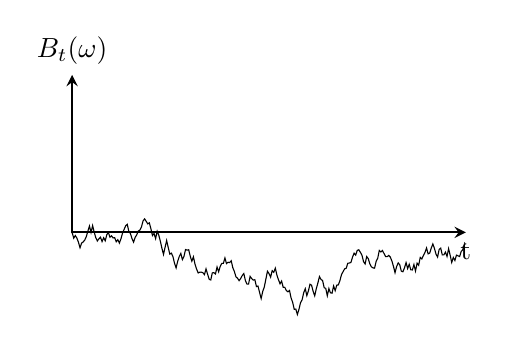
\begin{tikzpicture}[>=stealth, line cap=round]
\draw [thick, ->] (0,0) -- (0, 2)
  	node [sloped, above] {$B_t(\omega)$};
\draw [thick, ->] (0,0) -- (5,0)
 	node [below] {t};
\Emmett{250}{0.02}{0.1}{black}{}
\end{tikzpicture}
\caption{Some realisation of a stochastic process $X_t{(\omega)}$.}
\end{figure}

\noindent or ``realisation'' of the process. So, fix $t$ and consider a map $\omega \rightarrow X(\omega,t)$. For each fixed $t$, $X(\omega,t)$ would have some distribution (i.e. the distribution of the ``cross section'' of $X(\omega,t)$ for fixed $t$). \\
\\
\noindent Let $B \in \mathcal B(\mathbb R^d)$ and consider 
\begin{equation*}
X^{-1}_s(B) = \{\omega \in \Omega : X_s(\omega) \in B\}
\end{equation*}
Define 
\begin{equation*} 
\mathcal X_s = \{X^{-1}_s(B) : B \in \mathcal B(\mathbb R^d)\} \quad \text{(not necessarily a $\sigma$-algebra)}
\end{equation*}
\\
Then, let 
\begin{equation*} 
\mathcal F^X_t = \sigma(\mathcal X_s: 0 \leq s \leq t) \quad \text{(i.e. our $\sigma$-algebra generated by $\mathcal X_s$)}
\end{equation*}
\noindent Note that $\mathcal F^X_t$ contains $\mathcal F^X_s$ (i.e. $\mathcal F^X_s \subseteq \mathcal F^X_t$). We say that $(\mathcal F^X_t)_{t\geq0}$ is a \underline{filtration}, that is more information is releaved in our $\sigma$-algebra as we progress in $t$.

\subsection{Brownian Motion}

\begin{definition} A $d$-dimensional \underline{Brownian Motion} (BM) is a random walk/stochastic process $B_t$ with properties
\begin{enumerate}
	\item $B_0 =  \hat{0} \in \mathbb R^d$
	\item $B_t$ has independent increments, that is, for $0 = t_0 \leq t_1 \leq \cdots \leq t_n$,
		\begin{equation*}
			B_{t_1} - B_{t_0}, B_{t_2} - B_{t_1}, \cdots, B_{t_n} - B_{t_{n-1}}
		\end{equation*}
		are independent random variables.
	\item For $0 \leq s \leq t, B_t - B_s \sim N(0, (t - s)\mathbb I^d)$, where $\mathbb I^d$ is the $d$-dimensional identity matrix.
	\item {\bf The most important property is that it is} (almost surely) {\bf continuous}\footnote{$\mathbb P(\{\omega : B_0(\omega) = 0 \text{ and } t \mapsto B_t(\omega) \text{ is continuous}\}) = 1$}.
\end{enumerate}
\end{definition}

\begin{figure}[h!]
\centering
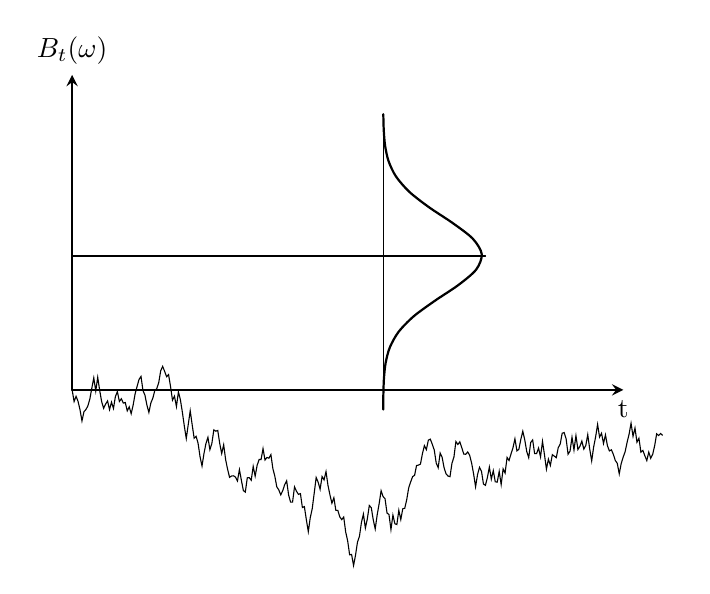
\begin{tikzpicture}[>=stealth, line cap=round]
\draw [thick, ->] (0,0) -- (0,4) node [sloped, above] {$B_t(\omega)$};
\draw [thick, ->] (0,0) -- (7,0) node [below] {t};
\draw [thick] plot [domain=-0.5:7, samples=20, smooth] ({3.95 + sqrt(0.5*pi)*exp(-0.5*pow((\x - 3.4),2))}, \x/2) coordinate (distribution-3);
\draw [] (3.95,0) -- (3.95,3.5);
\draw [] (0,1.7) -- (5.25,1.7);
\Emmett{300}{0.025}{0.2}{black}{}
\end{tikzpicture}
\caption{Intervals in one dimensional Brownian Motion are normally distributed with $\mu = 0$ and $\sigma^2 = (t - s)$.}
\end{figure}



\end{section}





























































\end{document}